% Make two column format for LaTex 2e
\documentclass[10pt,twocolumn,a4paper]{article}

% Use the following packages
\usepackage[utf8]{inputenc}     % Support for UTF-8
\usepackage{dcolumn}            % Align table columns on decimal point
\usepackage{graphicx}           % Include graphics
\usepackage{asymptote}          % Vector graphics language
\usepackage{listings}           % Pretty source code listings
\usepackage{url}                % Handle URLs better
\usepackage{amsmath}            % Extend mathematical typesetting

% Set dimensions of columns, gap between columns, and paragraph indent
\setlength{\textheight}{8.875in}
\setlength{\textwidth}{6.875in}
\setlength{\columnsep}{0.3125in}
\setlength{\topmargin}{0in}
\setlength{\headheight}{0in}
\setlength{\headsep}{0in}
\setlength{\parindent}{1pc}
\setlength{\oddsidemargin}{-.1875in}    % Centers the text
\setlength{\evensidemargin}{-.1875in}

% Add the period after section numbers, and adjust spacing
\newcommand{\Section}[1]{\vspace{-8pt}\section{\hskip -1em.~~#1}\vspace{-3pt}}
\newcommand{\SubSection}[1]{\vspace{-3pt}\subsection{\hskip -1em.~~#1}
\vspace{-3pt}}

% Global Asymptote definitions
\begin{asydef}
import three;
usepackage("bm");
texpreamble("\def\V#1{\bm{#1}}");
\end{asydef}

% Document
\begin{document}

% Make the title bold
\title{\bf The Right Arm Bias in ITF Taekwon-Do \\ Patterns Chon-Ji to Juche}

% Author information
\author{Bjørn Michelsen, III. Dan \\
  \texttt{<bjorn@bmichelsen.no>} \\
  \\
  ITF Tromsdalen School of Taekwon-Do \\
  Tromsø, Norway
  }

% Print date
\date{\today}

% Produce the title
\maketitle

% Sections
\section*{\centering Abstract}
\begin{em}

%An academic abstract typically outlines four elements germane to the completed work:

    %* The research focus (i.e. statement of the problem(s)/research issue(s) addressed);
    %* The research methods used (experimental research, case studies, questionnaires, etc.);
    %* The results/findings of the research; and
    %* The main conclusions and recommendations

  Todo.
\end{em}


\Section{Introduction}

  A \emph{pattern} in International Taekwon-Do Federation (ITF) is defined as
  a choreographed sequence of fundamental movements. These \emph{fundamental
  movements} are basic elements which represent an attack or defense against a
  specific target area, or a predetermined action of an attacker.

  Combined in a pattern, it allows the student to systematically deal with one
  or several imaginary opponents under various assumptions, using every
  available attacking and blocking tool from different directions. In
  addition, the techniques should also be evenly distributed between the left
  and the right side\cite{cyclo:vol1}.

  It has, however, recently been observed that a bias towards the right leg
  exist. The study by Gibbs\cite{rlb} show that there is a total of 152 kicks
  in patterns Chon-Ji to Tong-Il. 85 kicks are with the right leg, and 67
  kicks are with the left leg. This means that 56 \% of the kicks are with the
  right leg, and 44 \% with the left leg.

  The work by Gibbs focused on kicks in all patterns, whereas this article
  examines patterns Chon-Ji to Juche. Looking at kicks in said patterns using
  Gibbs' paper, we find that there are 72 kicks in total. 42 kicks are with
  the right leg, and 30 kicks are with the left leg. Roughly 58 \% of the
  kicks are with the right leg, and about 42 \% with the left. Thus, the right
  leg bias still holds.

  In this article we analyze hand techniques in patterns Chon-Ji to Juche
  using tags, and then report our findings of a right arm bias.


\SubSection{Tags}

  In a hierarchical and exclusive classification system, each object belong in
  one unambiguous category, which in turn is within another more general one.

  Take the hierarchy of folders in a computer file system, for example. How we
  choose to organize the folders reflects a decision concerning the relative
  importance of each characteristic\cite{golder:ct}.

  Folder names are in themselves informative, in that, like tags, they
  describe the information held within them\cite{jones:folders}. Furthermore,
  the way folder names relate to each other show a structural relationship
  between directories\cite{mathes:folk}.

  \emph{Tags}, on the other hand, are non-hierarchical descriptive terms,
  keywords or labels that is attached to an object for later retrieval
  \cite{golder:ct}\cite{huang:tt}\cite{shirky:ontology}.

  They are \emph{non-hierarchical} and \emph{inclusive}, which is to say that
  an object can be associated with a great variety of tags
  simultaneously\cite{golder:ct}. The \emph{descriptive terms},
  \emph{keywords} or \emph{labels} are metadata connected to a given object
  that describes a concept or type of information\cite{heymann:ccch}.


\SubSection{Tagging}

  \emph{Tagging} is the act of organizing a collection of objects into related
  groups\cite{shirky:ontology}.


\SubSection{Set Theory}
  A \emph{set} is a collection of distinct objects. It is ``a plurality
  thought of as a unit''\cite{hausdorff:sets}. \emph{Set theory}, then, is the
  branch of mathematics that studies sets.

  An object which has been tagged contains a collection, or a set, of tags.
  Each tag is an element of the set. The order of elements within the set is
  irrelevant, but each element can only occur once.

  For example, $\{1,5,8\}$ is a set with three elements: 1, 5 and 8.
  $\{5,8,1\}$ is the same set, since the order of the elements doesn't matter.
  $\{1,1,1\}$, however, is not a valid set because the element 1 occurs
  repeatedly. Elements in a set can contain strings as well, so $\{blocks,
  punches, strikes, thrusts\}$ is also a valid set.

  We usually denote a set by a capital letter for reference purposes. For
  instance, $S=\{1,5,8\}$.

  $a \in S$ denotes that the object $a$ is a member of the set $S$. If $a$
  is not a member of S, we write $a \notin S$.

  The \emph{union} of two sets $S$ and $T$ is the set

  \[
    S \cup T = \{x:x \in S \: or \: x \in T\}
  \]

  % Venn diagram, showing the union of two sets
  \input{venn_union.asy}

  This consists of those objects which lie in the set $S$ or in the set $T$,
  or in both. So,

  \[
    \{1, 2, 3\} \cup \{3, 4, 5\} = \{1, 2, 3, 4, 5\}
  \]

  The \emph{intersection} of two sets $S$ and $T$ is the set

  \[
    S \cap T = \{x:x \in S \: and \: x \in T\}
  \]

  % Venn diagram, showing the intersect of two sets
  \input{venn_intersect.asy}

  This consists of those objects which lie in both the set $S$ and the set
  $B$. So,

  \[
    \{1, 2, 3\} \cap \{2, 3, 4\} = \{2, 3\}
  \]

  The \emph{complement} of a set $T$ relative to a set $S$ is the set

  \[
    S - T = \{x:x \in S \: and \: x \notin T\}
  \]

  % Venn diagram, showing the complement of two sets
  \input{venn_complement.asy}

  This consists of those objects which lie in the set $S$ but not in the set
  $T$. So,

  \[
    \{1, 2, 3\} - \{2, 3, 4\} = \{1\}
  \]

  The \emph{symmetric difference} of the sets $S$ and $T$ is the set

  \[
    S \Delta T = \{x:(x \in S \: and \: x \notin T) \: or \: (x \in T \: and
    \: x \notin S)\}
  \]

  % Venn diagram, showing the symmetric difference of two sets
  \input{venn_difference.asy}

  This consists of those objects which lie either in one of the sets, but not
  in both. So,

  \[
    \{1, 2, 3\} \Delta \{2, 3, 4\} = \{1, 4\}
  \]


\Section{Method}

  In this section we describe where the data originates. Next we elaborate on
  the approach taken to register and investigate the dataset. Finally, we look
  at how each movement has been classified with emphasis on special cases.


\SubSection{The Data}

  Our data comes from two different sources. The terminology associated with
  pattern movements is from Taekwon-Do ITF Sonkal Praha\footnote{\url{http://
  sonkal.taekwondo.cz}}, and the English description of each movement is from
  the condensed encyclopedia\cite{cyclo:con}.

  The dataset is organized by pattern names. It contains a list of all
  techniques in patterns Chon-Ji to Juche. For each movement, the following
  data has been registered:

  \begin{enumerate}
    \item Movement number
    \item English description
    \item Terminology
    \item Tags
  \end{enumerate}


\SubSection{Approach}

  The movement number, together with the English description of each movement,
  was registered manually from the condensed encyclopedia. After reviewing and
  making minor corrections to the terminology, it too was added to the
  dataset.
  
  Suitable tags were then attached to every movement by first extracting
  keywords from their English description, and then adding more detailed tags
  while performing the pattern.

  We then defined the data models with DataMapper, an Object Relational
  Mapper\footnote{\url{http://www.datamapper.org}} (ORM) written in the Ruby
  programming language. The models are Ruby classes with properties and
  associations. Properties define field names and data types in the database,
  whereas the associations defines the relationships and cardinality between
  the models.

  Next we created a Ruby script that reads the dataset and automatically
  populates the database. It sets up associations between models, and adds the
  appropriate tags to every movement, as well as associations between movement
  and pattern.

  Tagging movements in such a formalized manner, and registering it in a
  database, enables us to retrieve the data we are interested in using
  concepts from set theory.


\SubSection{Classification}

  Classification was done by attaching metadata, in terms of tags, to each
  pattern movement.

  The first movement in Chon-Ji, for instance, is to ``[m]ove the left foot to
  B, forming a left walking stance toward B while executing a low block to B
  with the left forearm\cite{cyclo:vol1}.'' Removing the verbose parts of the
  description leaves us with:

  \[
    \{left \: walking \: stance, \: low \: block, \: left \: forearm\}
  \]

  Supplementing the above with more detailed tags gives us:

  \begin{align*}
    \{walking \: stance, \: left \: stance, \: low \: technique, \\
    left \: technique, \: block, \: forearm, \\
    outer \: forearm, normal \: motion\}
  \end{align*}

  Information about the stance type is presented first, followed by stance
  side (left, right or none where applicable --- for example a sitting
  stance), technique height (low, middle, high), technique side (left arm or
  right arm, it can also be both), direction of the technique (when needed),
  primary technique type (attack, block, kick), technique group (block, punch,
  strike, thrust), tool group (forearm, knife hand, finger etc.), tool (inner
  forearm, outer forearm, double finger etc.), and finally motion type (normal
  motion, slow motion, consecutive motion and so on).

  In most cases, applying tags to movements have been straightforward.
  However, there are movements that need special mention. These movements
  fall into two categories.

  The first category consist of movements where both arms are part of the
  technique by either forming the technique, or by being two separate
  techniques in a single movement.

  When both arms are used in one technique, the movement has been tagged with
  $\{left\_technique, \: right\_technique\}$ to reflect that both arms are
  needed for the technique, or that the movement contains two separate hand
  techniques.

  An example of a movement where both arms are required to form the technique
  can be found in the 13\textsuperscript{th} movement of Joong-Gun Tul, which
  is \emph{Gunnun so kyocha joomuk chukyo makgi}.

  When it comes to a movement with two separate hand techniques, the
  27\textsuperscript{th} movement of Joong-Gun Tul, being \emph{Nachuo so
  sonbadak noollo makgi}, serves as a good illustration.

  The implications of tagging movements with $\{left\_technique, \:
  right\_technique\}$ is that the total amount of hand techniques on either
  side are higher than what actually is the case. This flaw does not affect
  the bias we are investigating, though.

  The second category comprises ambiguous movements, and thus contain
  clarification on why certain tags were added.

  Below is a list of all the special cases from both categories.

\begin{itemize}
  \item
    \emph{Do-San Tul}
    \begin{itemize}
      \item
        {\bf Movement 13}, \emph{Gunnun so bakat palmok nopunde hechyo makgi},
        is tagged as a left and a right technique with $\{left\_technique, \:
        right\_technique\}$. This increases the total amount of blocks on both
        sides.
       \item
        {\bf Movement 17}, \emph{Gunnun so bakat palmok nopunde hechyo makgi},
        is tagged as a left and a right technique with $\{left\_technique, \:
        right\_technique\}$. This increases the total amount of blocks on both
        sides.
    \end{itemize}
  \item
    \emph{Yul-Gok Tul}
    \begin{itemize}
      \item
        {\bf Movement 24}, \emph{Gunnun so ap palkup bandae taerigi}, is
        tagged with $\{front\_strike\}$ due to the English description of
        striking with the right front elbow.
      \item
        {\bf Movement 27}, \emph{Gunnun so ap palkup bandae taerigi}, is
        tagged with $\{front\_strike\}$ due to the English description of
        striking with the left front elbow.
    \end{itemize}
  \item
    \emph{Joong-Gun Tul}
    \begin{itemize}
      \item
        {\bf Movement 8}, \emph{Gunnun so wipalkup taerigi}, is tagged
        $\{upper\_strike, \: upper\_elbow\}$ since the English description
        says that the movement is ``a right upper elbow strike.''
      \item
        {\bf Movement 10}, \emph{Gunnun so wipalkup taerigi}, is tagged
        $\{upper\_strike, \: upper\_elbow\}$ since the English description
        says that the movement is ``a left upper elbow strike.''
      \item
        {\bf Movement 11}, \emph{Gunnun so sang sewo jirugi}, is tagged as a
        left and right technique, with $\{left\_technique, \:
        right\_technique\}$. This increases the total amount of punches on
        both sides.
      \item
        {\bf Movement 12}, \emph{Gunnun so sang dwijibo jirugi}, is tagged as
        a left and right technique, with $\{left\_technique, \:
        right\_technique\}$. This increases the total amount of punches on
        both sides.
      \item
        {\bf Movement 13}, \emph{Gunnun so kyocha joomuk chukyo makgi}, is
        tagged as a left and a right technique with $\{left\_technique, \:
        right\_technique\}$. This increases the total amount of blocks on both
        sides.
      \item
        {\bf Movement 27}, \emph{Nachuo so sonbadak noollo makgi}, is tagged as
        a $\{middle\_technique, \: low\_technique\}$ because the left hand is
        in the middle section and the right hand, forming the pressing block,
        is in the low section of the body. The movement has, additionally, been
        tagged as a $\{right\_technique, \: left\_technique\}$ to reflect that
        two separate blocks are executed.
      \item
        {\bf Movement 29}, \emph{Nachuo so sonbadak noollo makgi}, is tagged as
        a $\{middle\_technique, \: low\_technique\}$ because the right hand is
        in the middle section and the left hand, forming the pressing block, is
        in the low section of the body. The movement has, additionally, been
        tagged as a $\{right\_technique, \: left\_technique\}$ to reflect that
        two separate blocks are executed.
    \end{itemize}
  \item
    \emph{Toi-Gae Tul}
    \begin{itemize}
      \item
        {\bf Movement 7}, \emph{Gunnun so kyocha joomuk noollo makgi}, is
        tagged as a left and a right technique with $\{left\_technique, \:
        right\_technique\}$. This increases the total amount of blocks on both
        sides.
      \item
        {\bf Movement 8}, \emph{Gunnun so sang sewo jirugi}, is tagged as a
        left and right technique, with $\{left\_technique, \:
        right\_technique\}$. This increases the total amount of punches on
        both sides.
      \item
        {\bf Movement 20}, \emph{Gunnun so}, has only the stance registered
        although the English description says to ``[e]xtend both hands upward
        as if to grab the opponent's head.''
      \item
        {\bf Movement 29}, \emph{Gunnun so kyocha joomuk noollo makgi}, is
        tagged as a left and a right technique with $\{left\_technique, \:
        right\_technique\}$. This increases the total amount of blocks on both
        sides.
    \end{itemize}
  \item
    \emph{Hwa-Rang Tul}
    \begin{itemize}
      \item
        {\bf Movement 24}, \emph{Gunnun so kyocha joomuk noollo makgi}, is
        tagged as a left and a right technique with $\{left\_technique, \:
        right\_technique\}$. This increases the total amount of blocks on both
        sides.
    \end{itemize}
  \item
    \emph{Choong-Moo Tul}
    \begin{itemize}
      \item
        {\bf Movement 11}, \emph{Gunnun sogi}, has only the stance registered
        as part of the terminology though the English description says to
        ``[e]xtend both hands upward as if to grab the opponent's head.''
      \item
        {\bf Movement 27}, \emph{Niunja so kyocha sonkal kaunde momcho makgi},
        is tagged as a left and a right technique with $\{left\_technique, \:
        right\_technique\}$. This increases the total amount of blocks on both
        sides.
    \end{itemize}
  \item
    \emph{Kwang-Gae Tul}
    \begin{itemize}
      \item
        {\bf Movement 21}, \emph{Nachuo so sonbadak noollo makgi}, is tagged as
        a $\{middle\_technique, \: low\_technique\}$ because the right hand is
        in the middle section and the left hand, forming the pressing block, is
        in the low section of the body. The movement has, additionally, been
        tagged as a $\{right\_technique, \: left\_technique\}$ to reflect that
        two separate blocks are executed.
      \item
        {\bf Movement 22}, \emph{Nachuo so sonbadak noollo makgi}, is tagged as
        a $\{middle\_technique, \: low\_technique\}$ because the right hand is
        in the middle section and the left hand, forming the pressing block, is
        in the low section of the body. The movement has, additionally, been
        tagged as a $\{right\_technique, \: left\_technique\}$ to reflect that
        two separate blocks are executed.
      \item
        {\bf Movement 31}, \emph{Gunnun so sang sewo jirugi}, is tagged as a
        left and right technique, with $\{left\_technique, \:
        right\_technique\}$. This increases the total amount of punches on
        both sides.
      \item
        {\bf Movement 32}, \emph{Gunnun so sang dwijibo jirugi}, is tagged as
        a left and right technique, with $\{left\_technique, \:
        right\_technique\}$. This increases the total amount of punches on
        both sides.
      \item
        {\bf Movement 36}, \emph{Gunnun so sang dwijibo jirugi}, is tagged as
        a left and right technique, with $\{left\_technique, \:
        right\_technique\}$. This increases the total amount of punches on
        both sides.
    \end{itemize}
  \item
    \emph{Po-Eun Tul}
    \begin{itemize}
      \item
        {\bf Movement 6}, \emph{Annun so ap joomuk noollo makgi}, consist of
        two blocks. The first is a ``pressing block with the left fore fist,''
        and the second one is a ``side front block with the right inner
        forearm.'' When searching, this movement will only register as one
        block.
      \item
        {\bf Movement 7}, \emph{Annun so ap joomuk noollo makgi}, consist of
        two blocks. The first is a ``pressing block with the right fore
        fist,'' and the second one is a ``side front block with the left inner
        forearm.'' When searching, this movement will only register as one
        block.
      \item
        {\bf Movement 8}, \emph{Annun so an palmok kaunde hechyo makgi}, is
        tagged as a left and a right technique with $\{left\_technique, \:
        right\_technique\}$. This increases the total amount of blocks on both
        sides.
      \item
        {\bf Movement 24}, \emph{Annun so ap joomuk noollo makgi}, consist of
        two blocks. The first is a ``pressing block with the right fore
        fist,'' and the second one is a ``side front block with the left inner
        forearm.'' When searching, this movement will only register as one
        block.
      \item
        {\bf Movement 25}, \emph{Annun so ap joomuk noollo makgi}, consist of
        two blocks. The first is a ``pressing block with the left fore fist,''
        and the second one is a ``side front block with the right inner
        forearm.'' When searching, this movement will only register as one
        block.
      \item
        {\bf Movement 26}, \emph{Annun so an palmok kaunde hechyo makgi}, is
        tagged as a left and a right technique with $\{left\_technique, \:
        right\_technique\}$. This increases the total amount of blocks on both
        sides.
    \end{itemize}

    Movements 6, 7, 24 and 25 for pattern Po-Eun also have the following tags
    attached:

  \begin{align*}
    \{sitting\_stance, \: low\_technique, \: high\_technique, \\
    left\_technique, \: right\_technique, \: block, \\
    pressing\_block, fore\_fist, \: forearm, \\
    inner\_forearm, \: side\_front\_block, \\
    continuous\_motion\}
  \end{align*}

  \item
    \emph{Ge-Baek Tul}
    \begin{itemize}
      \item
        {\bf Movement 1}, \emph{Niunja so kyocha sonkal kaunde momcho makgi},
        is tagged as a left and a right technique with $\{left\_technique, \:
        right\_technique\}$. This increases the total amount of blocks on both
        sides.
      \item
        {\bf Movement 7}, \emph{Gunnun so nopunde doo bandalson makgi}, is
        tagged as a left and a right technique with $\{left\_technique, \:
        right\_technique\}$. This increases the total amount of blocks on both
        sides.
      \item
        {\bf Movement 20}, \emph{Annun so gutja makgi}, is tagged as a left
        and a right technique with $\{left\_technique, \: right\_technique\}$.
        This increases the total amount of blocks on both sides.
      \item
        {\bf Movement 23}, \emph{Twimyo yopcha jirugi}, the height of the kick
        is not registered.
      \item
        {\bf Movement 24}, \emph{Gunnun so sang sewo jirugi}, is tagged as a
        left and right technique, with $\{left\_technique, \:
        right\_technique\}$. This increases the total amount of punches on
        both sides.
      \item
        {\bf Movement 25}, \emph{Gunnun so nopunde doo bandalson makgi}, is
        tagged as a left and a right technique with $\{left\_technique, \:
        right\_technique\}$. This increases the total amount of blocks on both
        sides.
      \item
        {\bf Movement 34}, \emph{Gunnun so sang sewo jirugi}, is tagged as a
        left and right technique, with $\{left\_technique, \:
        right\_technique\}$. This increases the total amount of punches on
        both sides.
      \item
        {\bf Movement 36}, \emph{Annun so gutja makgi}, is tagged as a left
        and a right technique with $\{left\_technique, \: right\_technique\}$.
        This increases the total amount of blocks on both sides.
    \end{itemize}
  \item
    \emph{Eui-Am Tul}
    \begin{itemize}
      \item
        {\bf Movement 5}, \emph{Gunnun so kyocha joomuk naeryo makgi}, is
        tagged as a left and a right technique with $\{left\_technique, \:
        right\_technique\}$. This increases the total amount of blocks on both
        sides.
      \item
        {\bf Movement 18}, \emph{Gunnun so kyocha joomuk naeryo makgi}, is
        tagged as a left and a right technique with $\{left\_technique, \:
        right\_technique\}$. This increases the total amount of blocks on both
        sides.
      \item
        {\bf Movement 27}, \emph{Gunnun so sonkal kaunde hechyo makgi}, is
        tagged as a left and a right technique with $\{left\_technique, \:
        right\_technique\}$. This increases the total amount of blocks on both
        sides.
      \item
        {\bf Movement 29}, \emph{Dwitbal so sang sonbadak naeryo makgi}, is
        tagged as a left and a right technique with $\{left\_technique, \:
        right\_technique\}$. This increases the total amount of blocks on both
        sides.
      \item
        {\bf Movement 32}, \emph{Gunnun so sonkal kaunde hechyo makgi}, is
        tagged as a left and a right technique with $\{left\_technique, \:
        right\_technique\}$. This increases the total amount of blocks on both
        sides.
      \item
        {\bf Movement 34}, \emph{Dwitbal so sang sonbadak naeryo makgi}, is
        tagged as a left and a right technique with $\{left\_technique, \:
        right\_technique\}$. This increases the total amount of blocks on both
        sides.
    \end{itemize}
  \item
    \emph{Choong-Jang Tul}
    \begin{itemize}
      \item
        {\bf Movement 18}, \emph{Gunnun so kyocha joomuk noollo makgi}, is
        tagged as a left and a right technique with $\{left\_technique, \:
        right\_technique\}$. This increases the total amount of blocks on both
        sides.
      \item
        {\bf Movement 19}, \emph{Moorup najunde apcha busigi}, is tagged with
        $\{front\_snap\_kick, \: knee\}$ because the English description says
        to perform ``a low front snap kick to C with the right knee.'' This
        has an effect on the total amount of low front snap kicks.
      \item
        {\bf Movement 24}, \emph{Dwitbal so sang sonbadak noollo makgi}, is
        tagged as a left and a right technique with $\{left\_technique, \:
        right\_technique\}$. This increases the total amount of blocks on both
        sides.
      \item
        {\bf Movement 38}, \emph{Gunnun so bandae gutja makgi}, is tagged as a
        left and a right technique with $\{left\_technique, \:
        right\_technique\}$.  This increases the total amount of blocks on
        both sides.
      \item
        {\bf Movement 40}, \emph{Gunnun so bandae gutja makgi}, is tagged as a
        left and a right technique with $\{left\_technique, \:
        right\_technique\}$.  This increases the total amount of blocks on
        both sides.
      \item
        {\bf Movement 41}, \emph{Gunnun so sang sonkal soopyong taerigi}, is
        tagged with $\{knife\_hand, \: twin\_knife\_hand\}$.
    \end{itemize}
  \item
    \emph{Juche Tul}
    \begin{itemize}
      \item
        {\bf Movement 1}, \emph{Annun so an palmok narani makgi}, is tagged as
        left and a right technique with $\{left\_technique, \:
        right\_technique\}$. This increases the total amount of blocks on
        both sides.
      \item
        {\bf Movement 4}, \emph{Waebal so bakat palmok narani makgi}, is
        tagged as a left and a right technique with $\{left\_technique, :\
        right\_technique\}$. This increases the total amount of blocks on both
        sides. The movement also has the tag $\{parallel\_block\}$ attached to
        it.
      \item
        {\bf Movement 13}, \emph{Annun so an palmok narani makgi}, is tagged
        as a left and a right technique with $\{left\_technique, \:
        right\_technique\}$. This increases the total amount of blocks on both
        sides.
      \item
        {\bf Movement 16}, \emph{Waebal so bakat palmok narani makgi}, is
        tagged as a left and a right technique with $\{left\_technique, :\
        right\_technique\}$. This increases the total amount of blocks on both
        sides. The movement also has the tag $\{parallel\_block\}$ attached to
        it.
      \item
        {\bf Movement 38}, \emph{Sasun so sang sonbadak chookyo makgi}, is
        tagged as a left and a right technique with $\{left\_technique, \:
        right\_technique\}$. This increases the total amount of blocks on both
        sides.
    \end{itemize}
\end{itemize}


\Section{Results}

  Our findings show that of 519 techniques, 256 (49 \%) are with the left arm
  and 263 (51 \%) with the right arm (Table \ref{tab:table1}). Looking at the
  total amount of techniques, only 7 techniques (about 1 \%) separates an even
  distribution to both sides.

  \begin{table}
    \centering
    \begin{tabular}{l|r|r} \hline \hline
      & Left Arm & Right Arm \\ \hline

      Blocks    & 148   & 133 \\
      Punches   &  60   &  71 \\
      Strikes   &  34   &  38 \\
      Thrusts   &  14   &  21 \\

      \hline
      \textbf{Total}   & \textbf{256}   & \textbf{263} \\
      \hline

    \end{tabular}
    \caption{Number of techniques per arm by category.}
    \label{tab:table1}
  \end{table}


\SubSection{Techniques by Category}

  In terms of category distribution, there are more blocks on the left side
  than there are on the right side. There are, therefore, more attacks on the
  right side, than on the left side (Figure \ref{fig:techniques_all}, Table
  \ref{tab:table2}).

  Independent on side or total, all technique categories follow the same
  pattern having most blocks, then punches, strikes and finally thrusts.

  \begin{table}
    \centering
    \begin{tabular}{l|r|r} \hline \hline
      & Left Arm & Right Arm \\ \hline

      Blocks    &  57.81 \%    &  50.57 \% \\
      Punches   &  23.44 \%    &  27.00 \% \\
      Strikes   &  13.28 \%    &  14.45 \% \\
      Thrusts   &   5.47 \%    &   7.98 \% \\

      \hline
      \textbf{Total}   & \textbf{100 \%}   & \textbf{100 \%} \\
      \hline

    \end{tabular}
    \caption{Percent distribution of techniques per arm by category.}
    \label{tab:table2}
  \end{table}

  % Distribution of techniques by category
  \begin{figure}
    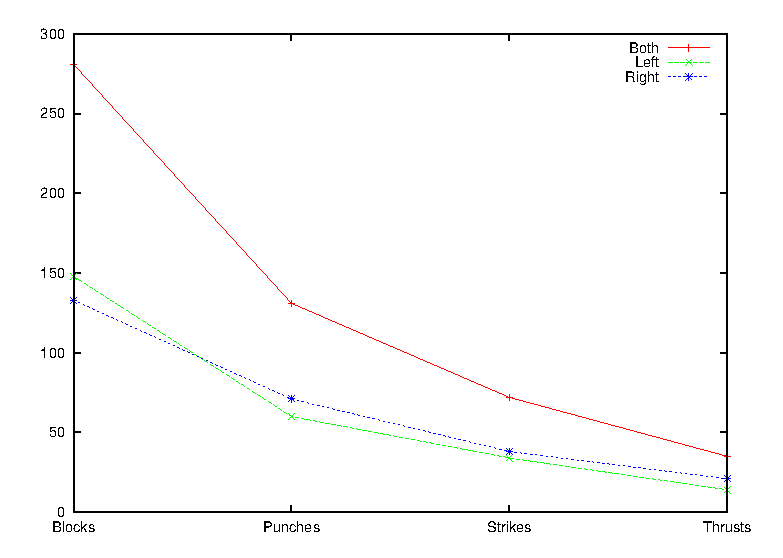
\includegraphics[scale=0.72]{data/gnuplot/eps/techniques_all}
    \caption{Distribution of techniques by category.}
    \label{fig:techniques_all}
  \end{figure}


\SubSection{Techniques by Height}

  % all techniques by height
  \begin{figure}
    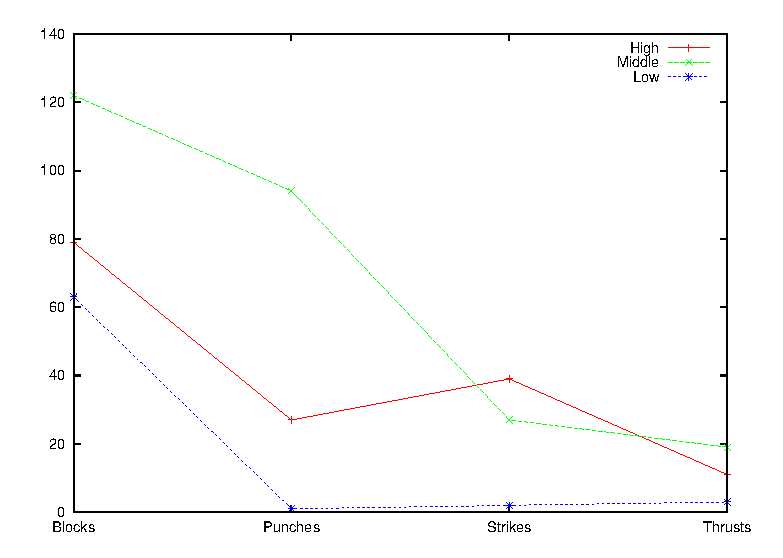
\includegraphics[scale=0.72]{data/gnuplot/eps/height_all}
    \caption{All techniques by height.}
    \label{fig:height_all}
  \end{figure}

  Techniques by height follow the same trend when looking at all techniques
  combined or techniques to either side. In general, there are more blocks
  than any other technique. Most of the techniques are in the middle section,
  although there is a greater occurrence of strikes in the high section, and
  very few attacks in the low section (Figure \ref{fig:height_all}).


\SubSection{Techniques by Stances}

  % All techniques by Walking, Sitting and L stances
  \begin{figure}
    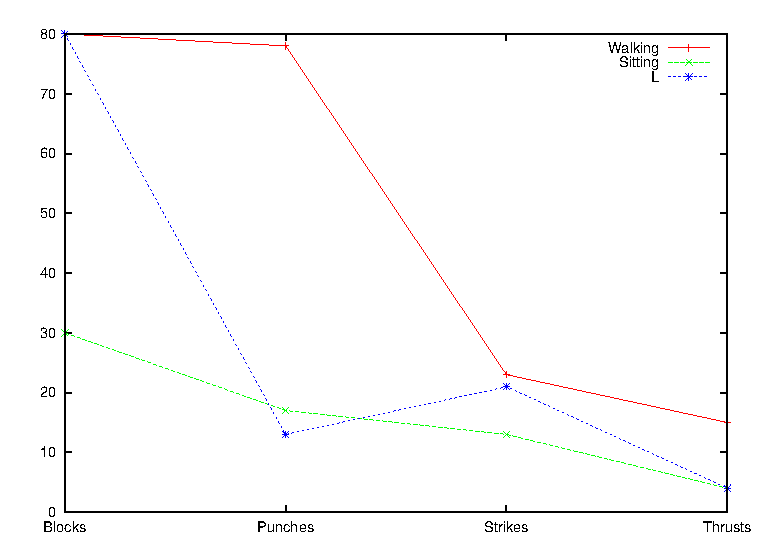
\includegraphics[scale=0.72]{data/gnuplot/eps/stances_all}
    \caption{All techniques by walking, sitting and L stances.}
    \label{fig:stances_all}
  \end{figure}

  Because most techniques are performed in walking, sitting and L stances, the
  graphs in this section have been split into two groups. One group shows the
  majority of techniques (84 \%), while the other visualize techniques
  performed in the remaining stances (16 \%).

  When looking at all techniques by walking stances, sitting stances and L
  stances (Figure \ref{fig:stances_all}), they roughly follow the same pattern
  on both sides. There are, however, two minor exceptions. Firstly, there are
  more strikes in L stances compared to walking stances on the left side.
  Secondly, there are more punches than blocks to the right side.

  % All techniques by stances except walking, sitting and L stances
  \begin{figure}
    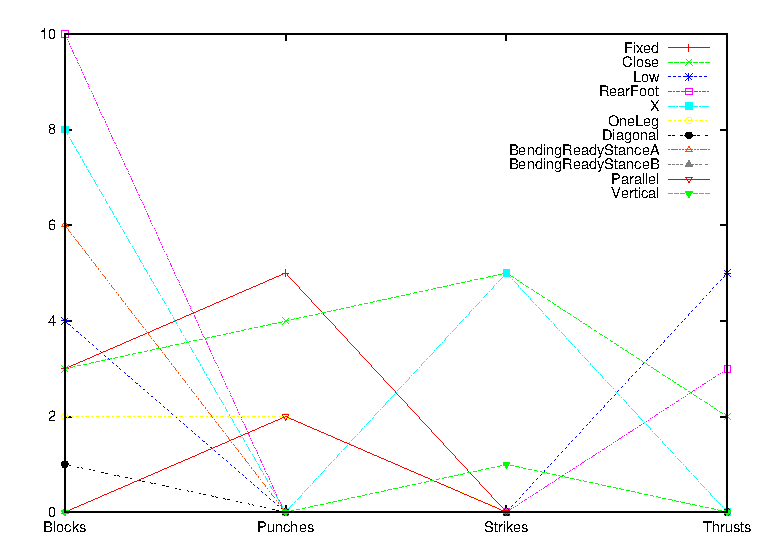
\includegraphics[scale=0.72]{data/gnuplot/eps/stances_not_wsl}
    \caption{All techniques by stances except walking, sitting and L stances.}
    \label{fig:stances_not_wsl}
  \end{figure}

  When we look at all techniques excluding the frequently used walking,
  sitting and L stances (Figure \ref{fig:stances_not_wsl}), we find that there
  is an even distribution of techniques except for the closed stance, the
  fixed stance and the vertical stance, which have more techniques to the
  right side (Figure \ref{fig:stances_left_not_wsl} than to the left (Figure
  \ref{fig:stances_right_not_wsl}.

  % Left techniques by stances except walking, sitting and L
  \begin{figure}
    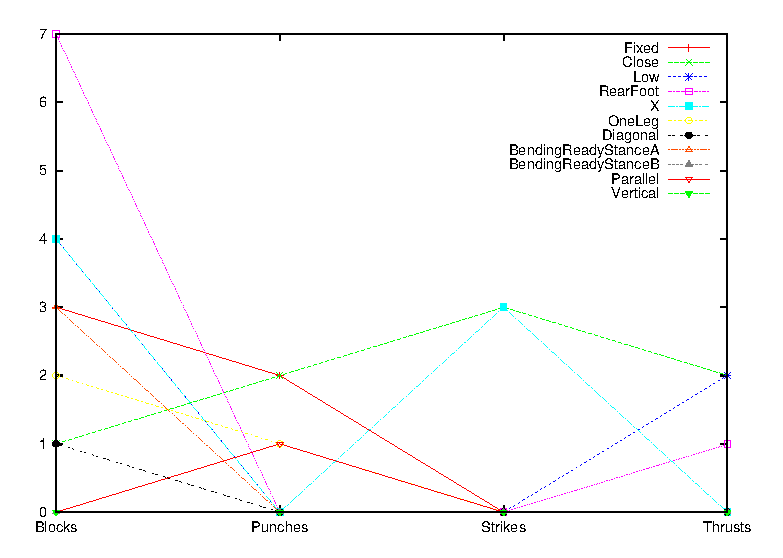
\includegraphics[scale=0.72]{data/gnuplot/eps/stances_left_not_wsl}
    \caption{Left techniques by stances except walking, sitting and L stances.}
    \label{fig:stances_left_not_wsl}
  \end{figure}

  % Right techniques by stances except walking, sitting and L
  \begin{figure}
    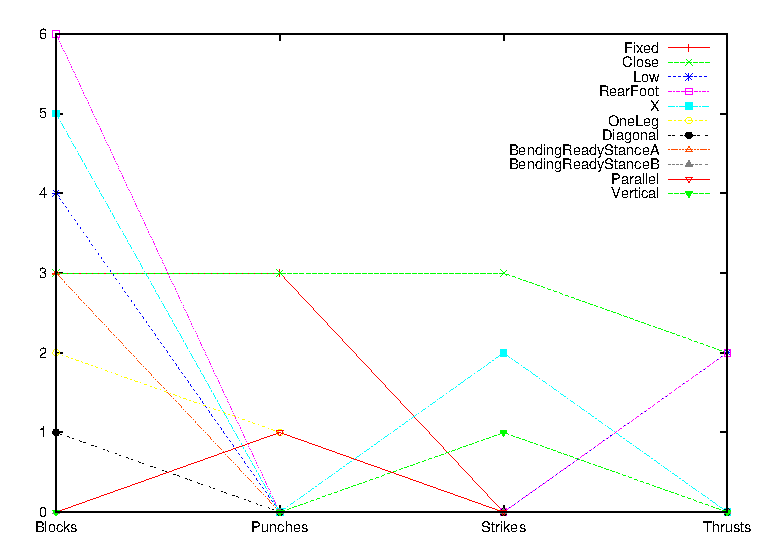
\includegraphics[scale=0.72]{data/gnuplot/eps/stances_right_not_wsl}
    \caption{Right techniques by stances except walking, sitting and L
    stances.}
    \label{fig:stances_right_not_wsl}
  \end{figure}

  There are some additional stances which needs special mentioning. The close
  stance is the only stance used by blocks, punches, strikes and thrusts. The
  parallel stance is only used for punches, whereas the vertical stance is
  only used for strikes. Only blocks are performed in the diagonal stance and
  the bending ready stance A. And finally, there are no techniques on the left
  side performed in the vertical stance.

  The total amount of techniques for both sides are 37 blocks and 34 attacks.
  Of all techniques on the left side, 59.5 \% are blocks, 40.46 \% are
  attacks. This means that there are 19.05 \% more blocks than attacks
  performed on that side. The right side follows the same pattern as the left,
  with more blocks than attacks. 57.51 \% of techniqes are blocks and 42.6 \%
  are attacks, meaning that there are 14.91 \% more blocks than attacks on the
  right side.


\SubSection{Techniques by Motion Type}

  % all techniques by motion type
  \begin{figure}
    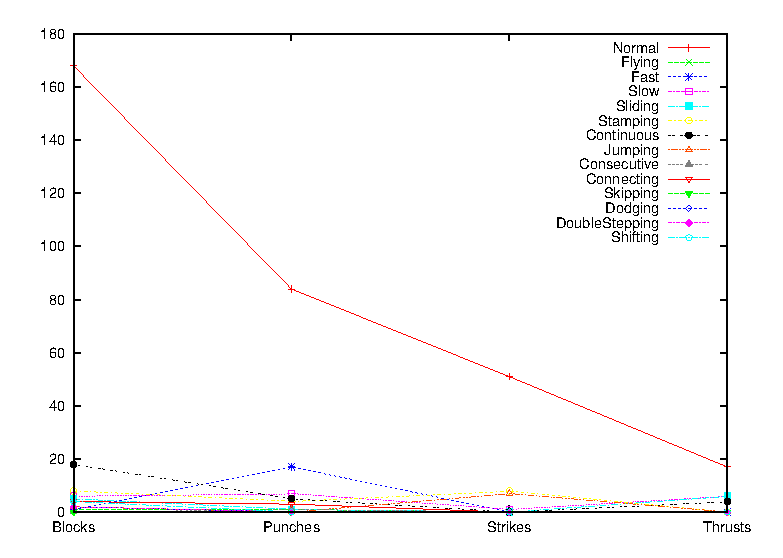
\includegraphics[scale=0.72]{data/gnuplot/eps/motion_all}
    \caption{All techniques by all motion types.}
    \label{fig:motion_all}
  \end{figure}

  There are 14 different motion types registered in our data set. The larger
  part of the techniques (76 \%) are performed in normal motion (Figure
  \ref{fig:motion_all}), followed by continuous motion (6 \%) and fast motion
  (4 \%).

  % all techniques by motion type except normal motion
  \begin{figure}
    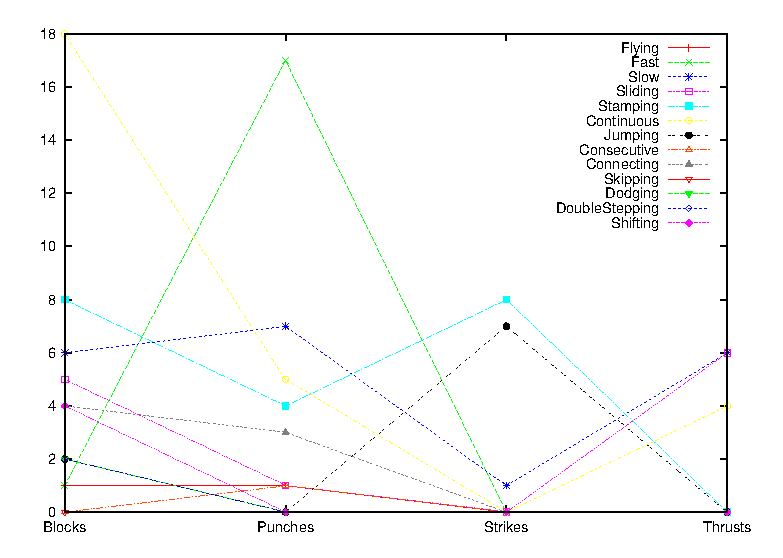
\includegraphics[scale=0.72]{data/gnuplot/eps/motion_all_not_n}
    \caption{All techniques by motion type except normal motion.}
    \label{fig:motion_all_not_n}
  \end{figure}

  Excluding normal motion, it is interesting to note the high presence of
  blocks in continuous motion, which alone amounts to 34 \% of blocks
  performed (Figure \ref{fig:motion_all_not_n}). Continuing with Figure
  \ref{fig:motion_all_not_n}, it shows that there is an abnormal number of
  punches performed in fast motion compared to other motion types.

  % left techniques by motion type except normal motion
  \begin{figure}
    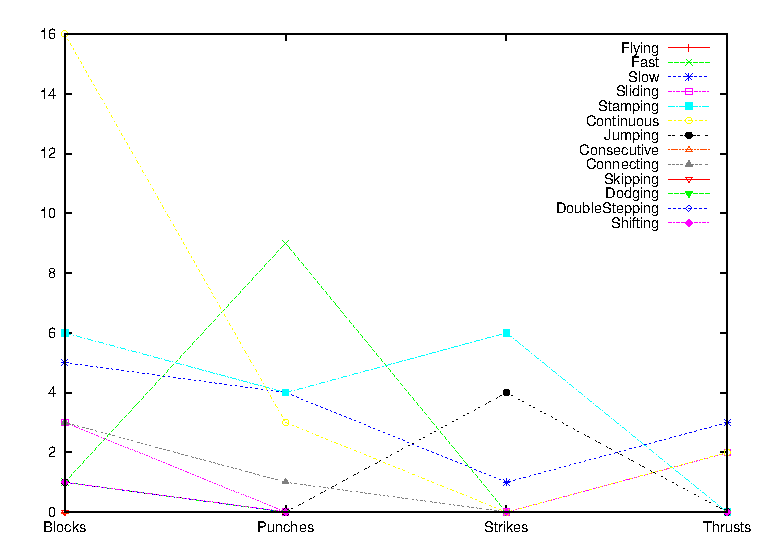
\includegraphics[scale=0.72]{data/gnuplot/eps/motion_left_not_n}
    \caption{Left techniques by motion type except normal motion.}
    \label{fig:motion_left_not_n}
  \end{figure}

  % right techniques by motion type except normal motion
  \begin{figure}
    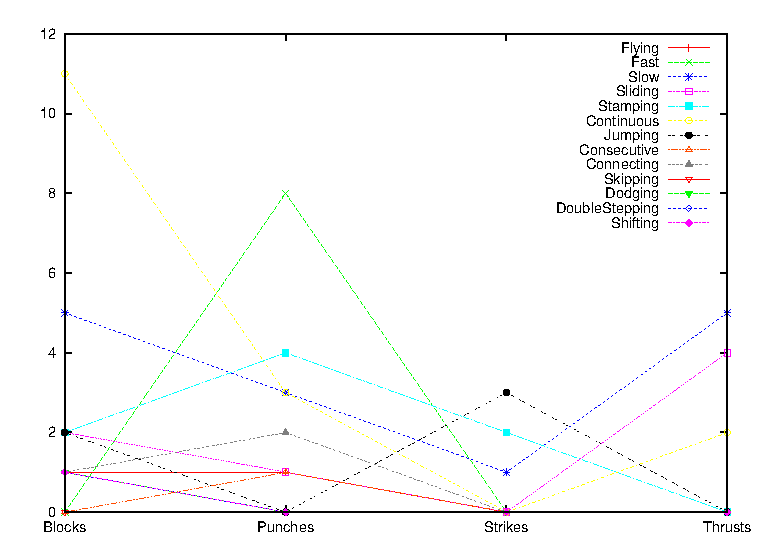
\includegraphics[scale=0.72]{data/gnuplot/eps/motion_right_not_n}
    \caption{Right techniques by motion type except normal motion.}
    \label{fig:motion_right_not_n}
  \end{figure}

  When examining the number of different motion types to either side, we find
  that there are more motion types on the right side, than on the left. The
  right side has flying motion and consecutive motion, in additon to motion
  types found on the left side. Also, there are more flying, slow, sliding and
  consecutive motions on the right side. However, there are more fast,
  stamping, continuous and connecting motions on the left side. Comparing the
  number of motion types on both sides reveals that there are equal amounts of
  slow, jumping, dodging, double stepping and shifting motions, although with
  different groups of techniques (Figures \ref{fig:motion_left_not_n},
  \ref{fig:motion_right_not_n}.



%\SubSection{Techniques by Patterns}


  %% all techniques by patterns
  %\begin{figure}
    %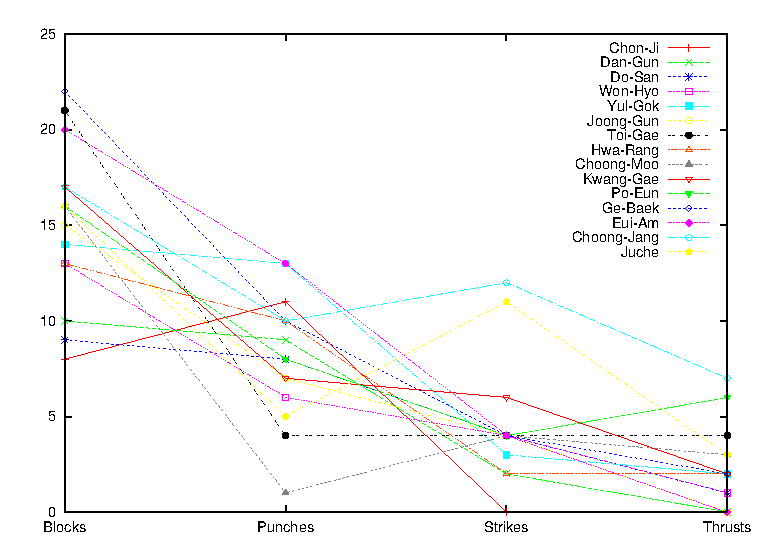
\includegraphics[scale=0.72]{data/gnuplot/eps/patterns_all}
    %\caption{All techniques by patterns.}
    %\label{fig:patterns_all}
  %\end{figure}

  %% left techniques by patterns
  %\begin{figure}
    %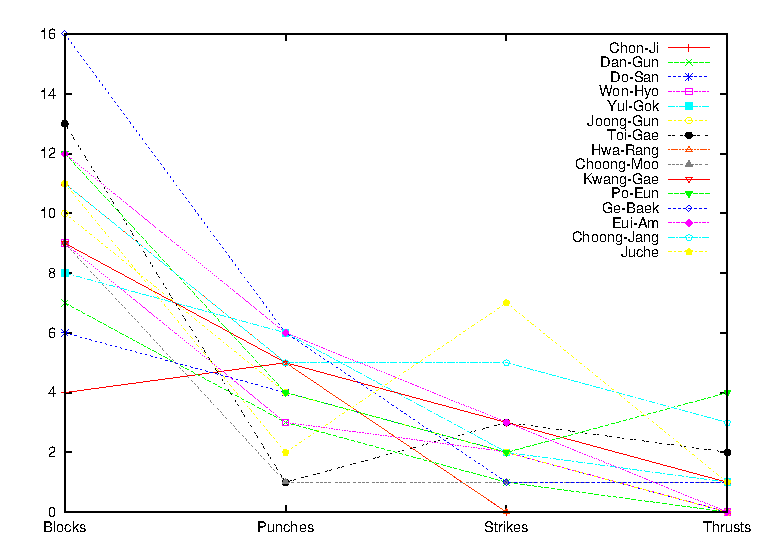
\includegraphics[scale=0.72]{data/gnuplot/eps/patterns_left}
    %\caption{Left techniques by patterns.}
    %\label{fig:patterns_left}
  %\end{figure}

  %% right techniques by patterns
  %\begin{figure}
    %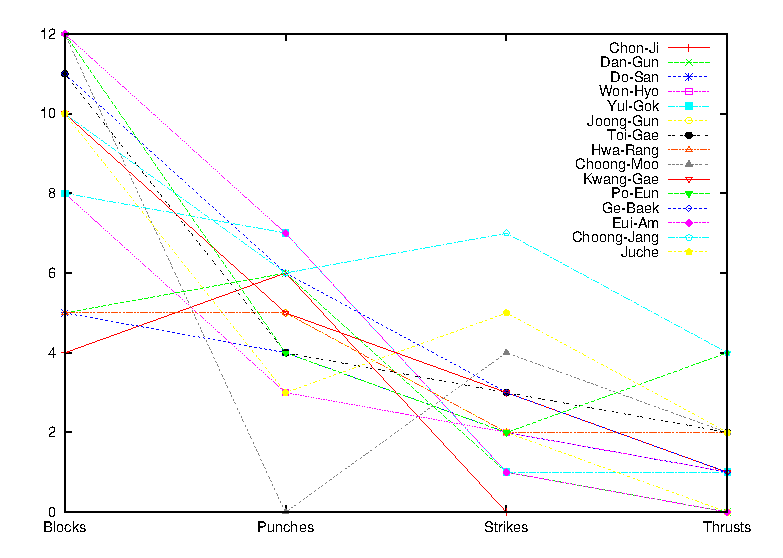
\includegraphics[scale=0.72]{data/gnuplot/eps/patterns_right}
    %\caption{Right techniques by patterns.}
    %\label{fig:patterns_right}
  %\end{figure}

  %% all techniques by black belt patterns
  %\begin{figure}
    %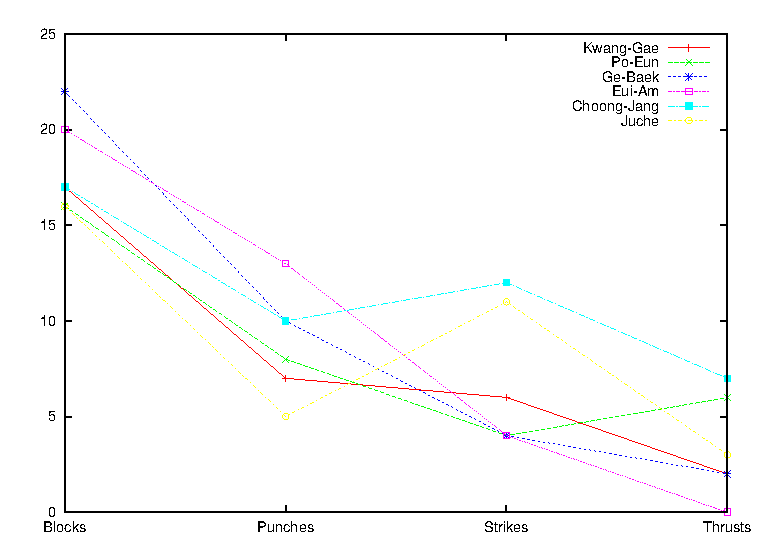
\includegraphics[scale=0.72]{data/gnuplot/eps/patterns_black_all}
    %\caption{All techniques by black belt patterns.}
    %\label{fig:patterns_black_all}
  %\end{figure}


  %% left techniques by black belt patterns
  %\begin{figure}
    %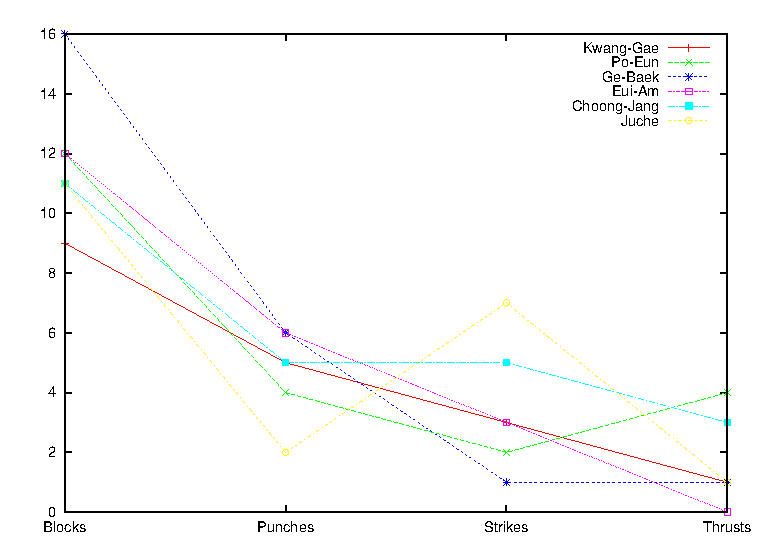
\includegraphics[scale=0.72]{data/gnuplot/eps/patterns_black_left}
    %\caption{Left techniques by black belt patterns.}
    %\label{fig:patterns_black_left}
  %\end{figure}

  %% right techniques by black belt patterns
  %\begin{figure}
    %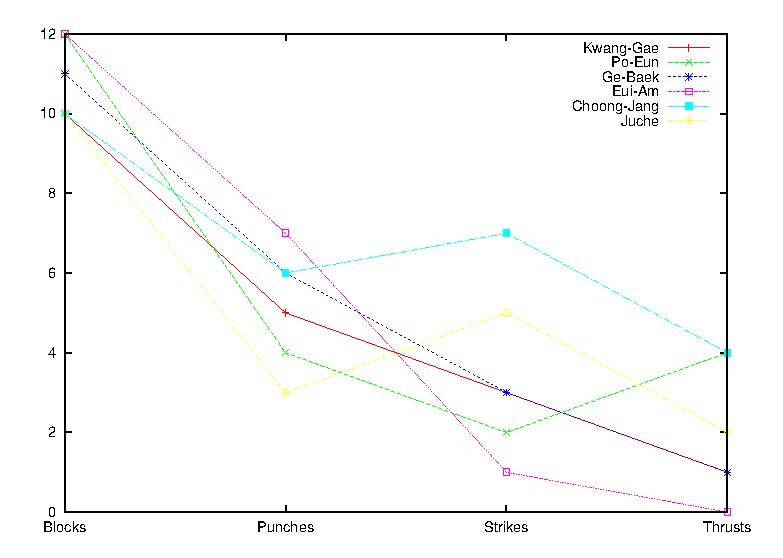
\includegraphics[scale=0.72]{data/gnuplot/eps/patterns_black_right}
    %\caption{Right techniques by black belt patterns.}
    %\label{fig:patterns_black_right}
  %\end{figure}


  %% all techniques by color belt patterns
  %\begin{figure}
    %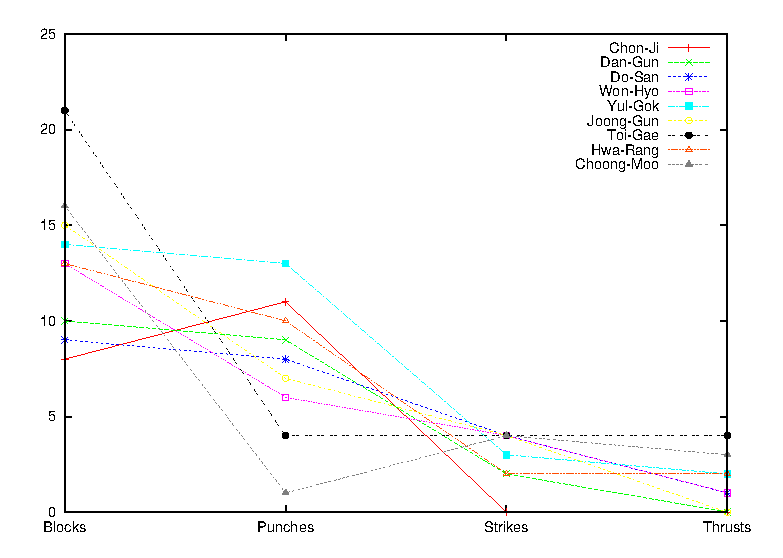
\includegraphics[scale=0.72]{data/gnuplot/eps/patterns_color_all}
    %\caption{All techniques by color belt patterns.}
    %\label{fig:patterns_color_all}
  %\end{figure}


  %% left techniques by color belt patterns
  %\begin{figure}
    %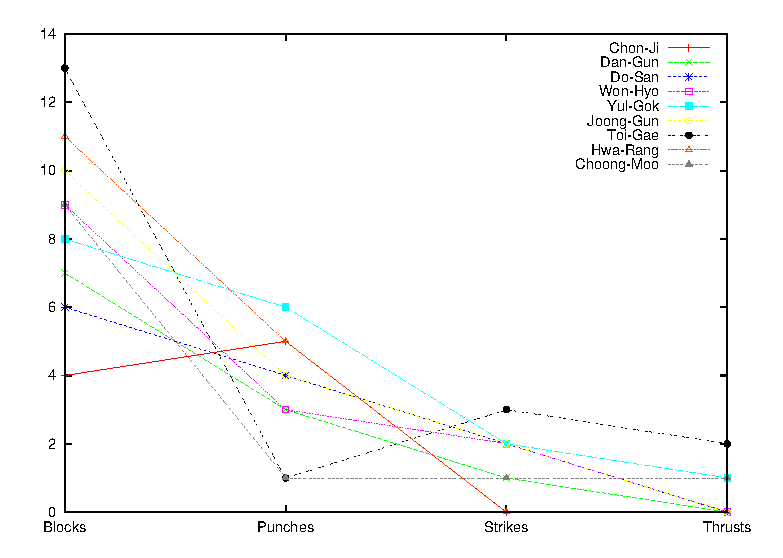
\includegraphics[scale=0.72]{data/gnuplot/eps/patterns_color_left}
    %\caption{Left techniques by color belt patterns.}
    %\label{fig:patterns_color_left}
  %\end{figure}

  %% right techniques by color belt patterns
  %\begin{figure}
    %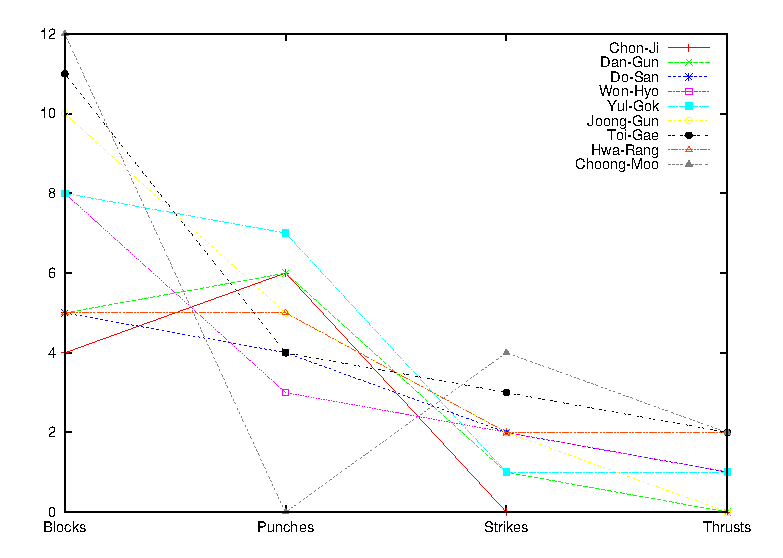
\includegraphics[scale=0.72]{data/gnuplot/eps/patterns_color_right}
    %\caption{Right techniques by color belt patterns.}
    %\label{fig:patterns_color_right}
  %\end{figure}












%\Section{Conclusions}

%What are the implications of your answer? Is it going to change the
%world (unlikely), be a significant ``win'', be a nice hack, or simply
%serve as a road sign indicating that this path is a waste of time (all
%of the previous results are useful). Are your results general,
%potentially generalizable, or specific to a particular case?


% Is it possible to say anything about why there are more techniques with the
% right hand, than with the left?

% Observation: Kicks happen between stances

% Future research
%   level of detail (ex. how each technique is divided per stance to say
%   something about what stance is more suited for a technique, or to show a
%   certain technique in a less/not used stance during step sparring to an
%   understanding of techniques beyond patterns

% {left_technique, right_technique} should probably have been tagged
% {both_hands} as well.

% Link to the source code.

% Movements with several blocks should have a tag indicating that there are
% more than one block in the movement.

% Unnumbered section (note the '*')
%\section*{Acknowledgments}

  % Thanks to Master Nicolaisen (VII. Dan) for pointing out that I already had
  % found a problem statement when I was still looking for one
  %
  % Odd-Magne Hansen (III. Dan) for helping me with the terminology, and
  % general feedback
  %Todo.










% References
\begin{thebibliography}{99}
    \small  % Use 9 point text

    \bibitem{cyclo:vol1}
      Gen. Choi Hong Hi,
      \emph{Encyclopedia of Taekwon-Do}, Vol. 1,
      International Taekwon-Do Federation, 1993.

    \bibitem{cyclo:con}
      Gen. Choi Hong Hi,
      \emph{Taekwon-Do (the Korean Art of Self-Defence)}, Fifth Edition,
      International Taekwon-Do Federation, 1999.

    \bibitem{rlb}
      M. Gibb,
      \emph{Right Leg Bias in Patterns}, 2009.
      \url{http://visiontkd.co.uk/assetshome/pdf/Rightlegbias.pdf}

    \bibitem{golder:ct}
      S. A. Golder, B. A. Huberman,
      \emph{The Structure of Collaborative Tagging Systems}, 2005.
      \url{http://www.hpl.hp.com/research/scl/papers/tags/tags.pdf}

    \bibitem{heymann:ccch}
      P. Heymann, H. Garcia-Molina,
      \emph{Collaborative Creation of Communal Hierarchical Taxonomies in
      Social Tagging Systems}, 2006.
      \url{http://ilpubs.stanford.edu:8090/775/1/2006-10.pdf}

    \bibitem{hausdorff:sets}
      F. Hausdorff,
      \emph{Set theory},
      Chelsea Publishing Company, 1991.

    \bibitem{huang:tt}
      J. Huang, K. M. Thornton, E. N. Efthimiadis,
      ``Conversational Tagging in Twitter,''
      \emph{Hypertext}, pp. 173-177, 2010.

    \bibitem{jones:folders}
      W. Jones, A. J. Phuwanartnurak, R. Gill, H. Bruce,
      \emph{Don't Take My Folders Away! Organizing Personal Information to Get
      Things Done}, 2005.
      \url{https://dlib.lib.washington.edu/dspace/bitstream/handle/1773/2031/
           Don%27t%20take%20my%20folders%20away%2c%20current.pdf?sequence=2}

    \bibitem{mathes:folk}
      A. Mathes,
      ``Folksonomies -- Cooperative Classification and Communication Through
      Shared Metadata,''
      \emph{Computer Mediated Communication, LIS590CMC}, 2004.

    \bibitem{shirky:ontology}
      C. Shirky,
      \emph{Ontology is Overrated: Categories, Links, and Tags}, 2005.
      \url{http://www.shirky.com/writings/ontology_overrated.html}

\end{thebibliography}

\end{document}
